\large{
Di seguito saranno viste le varie operazioni eseguibili dall'utente sull'editor. Per comodità per il lettore esse saranno divise nelle tre sezioni di seguito riportate:
\begin{itemize}
	\item \textbf{creazione} di un oggetto, di un grafo clusterizzato mediante file esterni o templates;
	\item \textbf{modifica} di un oggetto, aggiunta di informazioni o sostituzione di un attributo;
	\item \textbf{navigazione} all'interno del grafo creato; 
	\item \textbf{semplificazione} del grafo clusterizzato; 
\end{itemize}
Prima di passare alla descrizione dettagliata delle varie operazioni è necessario un focus sull'operazione di disegno del grafo nella graph-view in quanto questa è l'operazione che il sistema esegue ogni qual volta venga creato o modificato un oggetto sia della struttura dati che della sua rappresentazione.
\section{disegno dei dati}
Quasi tutte le operazioni di creazione o di modifica portano ad un cambiamento importante dei dati e quindi si ha la necessità di un costante cambiamento della loro visualizzazione. Ogni volta che l'utente esegue un cambiamento o l'aggiunta di un oggetto come mostrato schematicamente nella \figurename~\ref{fig:redraw} il sistema passerà ad effettuare una operazione di disegno dei dati per poi dare di nuovo il controllo all'utente.
\begin{figure}[!htb]
	\begin{center}
		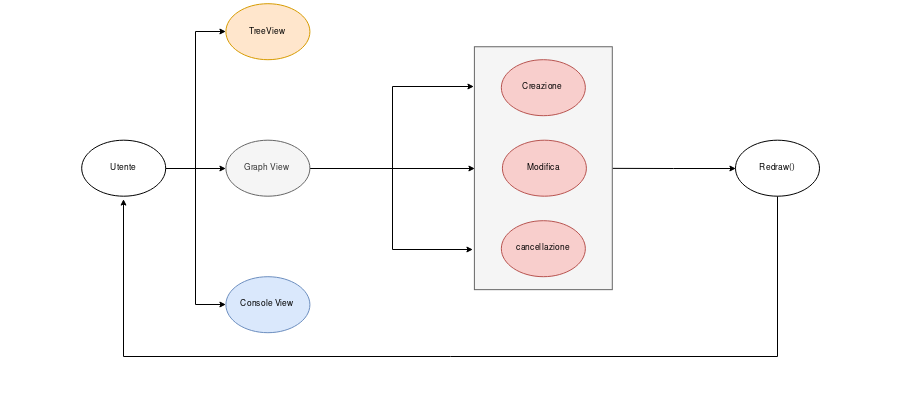
\includegraphics[width=1 \linewidth]{figure/redraw}
	\end{center}
	\caption{Schema dell'impiego della funzione di disegno dei dati \label{fig:redraw}}
\end{figure}
\newline
Quando questa operazione viene eseguita il sistema elimina completamente la sola visualizzazione degli svg lasciando però inalterato l'svg principale \#cgraph e ridisegnando con i cambiamenti effettuati nuovamente i dati creati o importati. Ricordando poi che si sta operando con un modello Node-link con una rappresentazione spring-embedding una volta ridisegnati i dati si passerà all'aggiunta delle forze fisiche, che controlleranno il movimento e la rappresentazione degli oggetti, eseguita mediante le funzionalità di D3. Ogni cluster di livello $l$ avrà dunque:
\begin{itemize}
	\item una forza attrattiva direzionata verso il centro dello stesso esclusivamente per i nodi prenenti nel suo attributo \textit{nodes};
	\item una forza repulsiva verso gli altri cluster dello stesso livello $l$; 
	\item una forza attrattiva direzionata verso il centro dello stesso esclusivamente per i cluster di livello inferiore presenti nel suo attributo \textit{cildren};
\end{itemize}
Ogni nodo invece avrà:
\begin{itemize}
	\item una forza attrattiva direzionata verso il centro del cluster di appartenenza;
	\item una forza repulsiva verso gli altri nodi;
\end{itemize}
Queste forze sono mostrate schematicamente nella \figurename~\ref{fig:springExample} in cui ogni vettore rappresenta la forza attrattiva nel caso in cui il verso sia entrante o repulsiva nel caso in cui il verso sia uscente.\\
Come si nota le forze in gioco sono molteplici e il ricalcolo della condizione di equilibrio risulta comunque pesante a livello di complessità computazionale temporale.
\begin{figure}[!htb]
	\begin{center}
		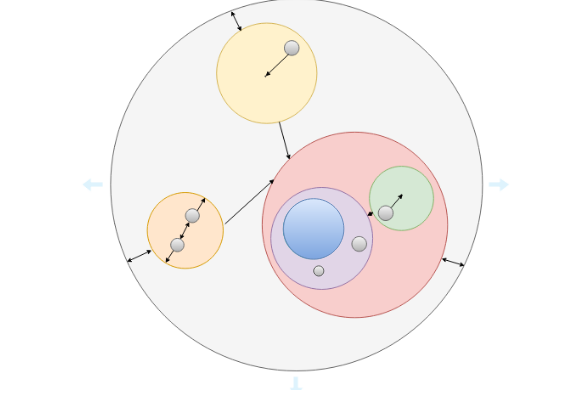
\includegraphics[width=1 \linewidth]{figure/springExample}
	\end{center}
	\caption{Esempio delle forze attrattive e repulsive utilizzate in fase di disegno \label{fig:springExample}}
\end{figure}
Una volta definita l'operazione di disegno degli oggetti da visualizzare è ora possibile procedere a definire come le primitive di interazione e le operazioni di semplificazione sono state impiegate nel sistema in esempio.
\newpage
\section{creazione}
Iniziando una sessione di lavoro l'utente ha la possibilità come già accennato di cominciare a creare e rappresentare un grafo clusterizzato oppure di importare dei dati per poterne avere solo la loro visualizzazione. L'import può essere eseguito mediante dati definibili tabellari provenienti da file con estensione \textit{.Json}.\\
%%% CITARE JSON.COM O ROBA SIMILE !!!
Si ricorda, prima di procedere, che il JSON (JavaScript Object Notation) è un formato di scambio dati di facile lettura e scrittura, di generazione e analisi per il calcolatore. Si basa su un sottoinsieme dello standard di programmazione JavaScript ECMA-262 3a edizione del dicembre 1999. JSON è un formato di testo che è completamente indipendente dal linguaggio ma utilizza convenzioni familiari ai programmatori della famiglia di linguaggi C, tra cui C, C ++, C \#, Java, JavaScript, Perl, Python e molti altri. Queste proprietà rendono JSON un linguaggio di scambio dati ideale.\\
JSON è costruito su due strutture:
\begin{itemize}
	\item Una raccolta di coppie nome / valore. In vari linguaggi, questo viene realizzato come oggetto, record, struct, dizionario, tabella hash, elenco con chiave o array associativo;
	\item Un elenco ordinato di valori che è realizzato come una matrice, un vettore o una sequenza. 
\end{itemize} 
Mediante un bottone di import è dunque possibile caricare un file json personale creato secondo la struttura fissa mostrata nella \figurename~\ref{fig:json} e passare questi dati al sistema per crearne la rappresentazione associata.\\
\begin{figure}[!htb]
	\begin{center}
		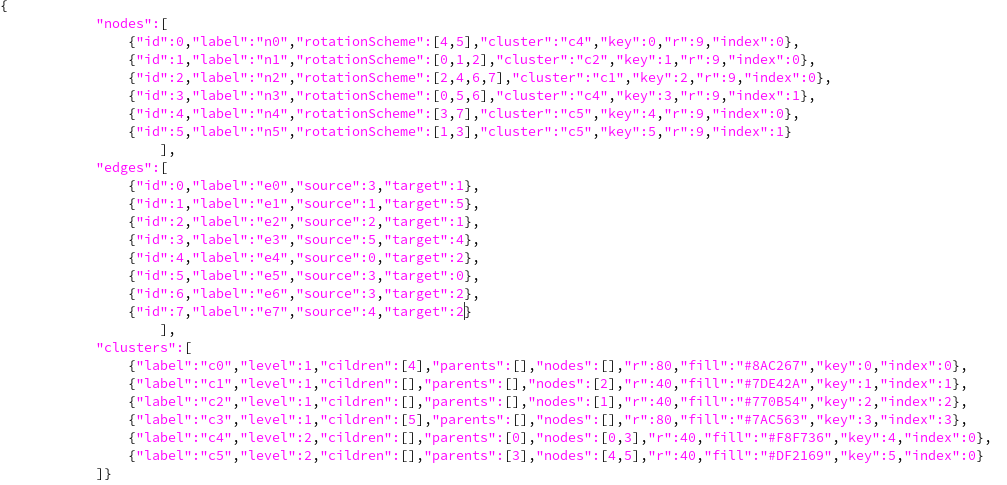
\includegraphics[width=1 \linewidth]{figure/json}
	\end{center}
	\caption{Esempio di file json per l'import di un grafo clusterizzato \label{fig:json}}
\end{figure}
\newline
In qualunque momento durante una sessione di lavoro è inoltre possibile l'export del grafo su cui si sta lavorando. In particolare l'utente ha due possibilità di salvataggio: della struttura o della visualizzazione. La prima e più importante è riferita all'export dei dati mediante file json che potranno essere poi ricaricati e riutilizzati per una sessione di lavoro futura. La seconda invece è riferita alla possibilità di salvaggio della rappresentazione dei dati mediante file con estenzione \textit{.PNG}. Si ricorda inoltre che il PNG (Portable Network Graphics) è un formato di file per memorizzare immagini. 
Ogni qualvolta che si sceglie di utilizzare l'import di un file esterno il sistema andrà prima ad eliminare tutto ciò che fa parte della sessione di lavoro su cui l'utente sta lavorando. In questo modo il sistema potrà importare i dati richiesti e procedere con la rappresentazione degli stessi.\\
Non avendo a disposizione file json per l'import dei dati o volendo semplicemente cominciare una sessione di lavoro non da una semplice pagina bianca l'utente ha a disposizione dei modelli predefiniti su cui potrà cominciare il lavoro ed andare a modificare a piacimento. I modelli non rappresentano solamente la visualizzazione in se ma si basano su dati tabellari. Esattamente come per l'import di file json anche l'utilizzo di modelli con un algoritmo simile a quello mostrato nella \figurename~\ref{fig:viewAlg}. In altre parole ogni qual volta l'utente chiede al sistema di creare un modello questo risponde eliminando tutta la sessione di lavoro ed inizializzando nuovamente con i dati definiti durante la richiesta di creazione mediante il modello scelto. Di default all'inizio di una sessione utente il sistema presenterà, come visto nella \figurename~\ref{fig:interfaccia}, una pagina di lavoro vuota proprio per lasciare all'utente la scelta non solo di tipologia di dati da poter creare ma anche della loro posizione sul piano di lavoro. Questo andrà però a pregiudicare il fatto che il conseguimento di una buona visualizzazione sarà compito dell'utente.\\
A prescindere dalla scelta di importare dati, utilizzare modelli o cominciare da un grafo vuoto, l'utente avrà la possibilità di inserire cluster, nodi e archi. È consigliabile seguire un criterio, quando possibile, nella creazione degli oggetti. Un buon metodo di creazione è quello che applica una strategia di discesa dell'albero di inclusione top-down partendo dunque dalla creazione dei cluster di livello uno, fino ad arrivare a quelli più in profondità per poi passare alla creazione delle foglie dell'albero, ovvero dei nodi terminando con gli archi. Ovviamente questa non è una regola e non pregiudica la creazione di un grafo ma è un buon principio per la visualizzazione che un utente dovrebbe seguire. Per questo ed altri motivi sono stati realizzati dei messaggi di errore che aiutano l'utente e lo indirizzano verso l'approccio sopra definito. Supponendo ad esempio che l'utente abbia creato due cluster di livello uno ed un nodo all'interno di uno dei due e dia al sistema l'input per poter cominciare la creazione di archi esso risponderà con il messaggio di errore mostrato in \figurename~\ref{fig:erroreArco}.
\begin{figure}[!htb]
	\begin{center}
		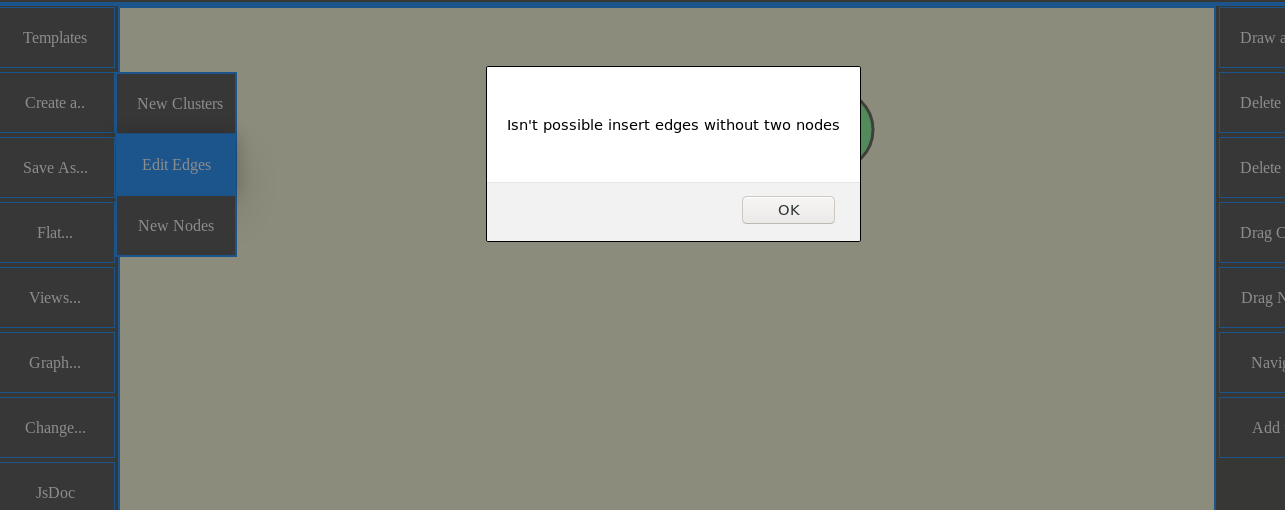
\includegraphics[width=0.8 \linewidth]{figure/erroreArco}
	\end{center}
	\caption{Messaggio di errore per il tentativo di creazione di un arco senza due nodi\label{fig:erroreArco}}
\end{figure}
\newline
Ogni volta che l'utente creerà un oggetto all'interno del piano di lavoro il sistema risponderà prima aggiornando la struttura dati a cui la visualizzazione fa riferimento ed andrà poi a creare nuovamente la loro rappresentazione. Una volta creati i cluster di un livello l'utente potrà creare i figli degli stessi. Recepita questa richiesta il sistema andrà ad aggiornare le strutture dati inizializzando il nuovo oggetto e collegandolo, con gli attributi visti nella \figurename~\ref{fig:clusterClass}, al cluster genitore.
Infine per quando riguarda la creazione degli archi all'utente basterà selezionare un nodo che sarà definito sorgente e un nodo destinazione per collegarli. Si è scelto di non utilizzare linee dritte nella rappresentazione ma curvate di modo da evitare qualora possibile intersezioni tra essi come si concerne ad un grafo planare anche se è a discrezione dell'utente il poter definire un grafo in cui gli archi possono incrociarsi o meno. Nella figura \figurename~\ref{fig:archi} è mostrato l'impiego di un gran numero di archi che tra loro non vanno ad intersecarsi al contrario di come sarebbe successo utilizzando linee rette.
\begin{figure}[!htb]
	\begin{center}
		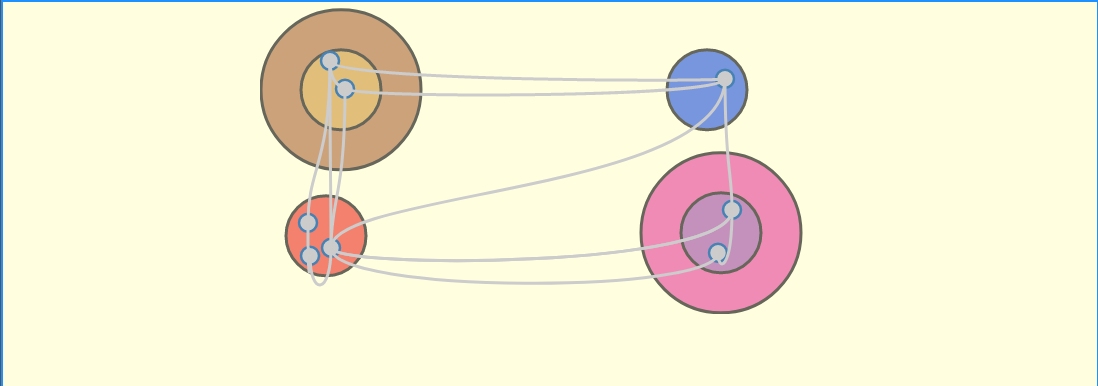
\includegraphics[width=0.8 \linewidth]{figure/archi}
	\end{center}
	\caption{Esempio di planarità nella rappresentazione di un grafo clusterizzato\label{fig:archi}}
\end{figure}

\section{modifica}
Il sistema lascia una buona libertà all'utente per quanto concerne la modifica degli oggetti le cui operazioni saranno viste nel dettaglio di seguito. \\
Per quanto riguarda gli oggetti visualizzati, che sono stati creati o importati durante la sessione di lavoro, l'utente ha la possibilità di spostamento sia di un oggetto cluster che di un nodo esattamente come richiesto dai principi espressi nel capitolo relativo alle primitive di interazione.
Essendo l'utente finale non esente da possibili errori di creazione degli oggetti è stata realizzata una funzione per la cancellazione di oggetti.Si riporta, in maniera semplificata, nella \figurename~\ref{fig:delete} l'algoritmo di eliminazione di un oggetto.
\begin{figure}[!htb]
	\begin{center}
		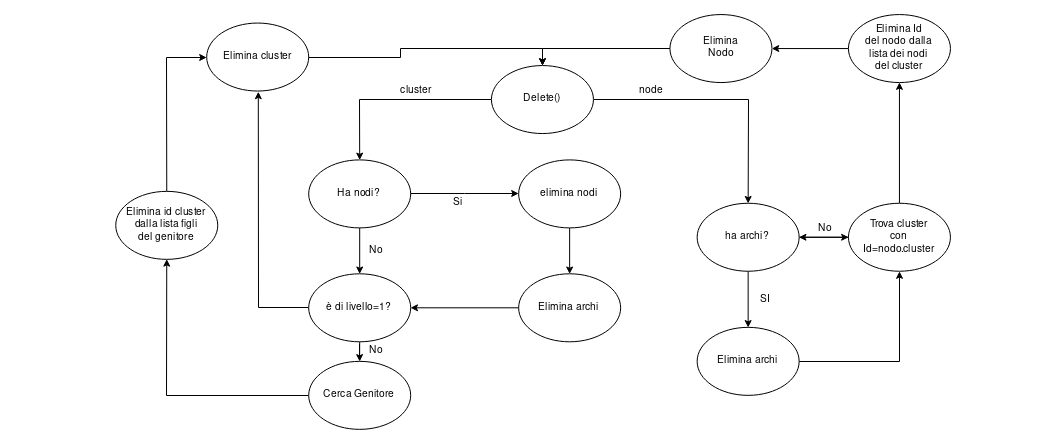
\includegraphics[width=1 \linewidth]{figure/delete}
	\end{center}
	\caption{algoritmo di cancellazione di un oggetto\label{fig:delete}}
\end{figure}
\newline
Oltre alle operazioni di cancellazione e spostamento l'utente ha la libertà di assegnare valori diversi da quelli di default per colori e raggio agli oggetti del grafo. In particolare, ricordando che il raggio di un cluster è definito come un valore di default $k_c$ moltiplicato per il numero e all'entità degli oggetti mentre quello di un nodo è un semplice valore $k_n$, l'utente potrà andare a modificare la dimensione di questi due valori indicando al sistema la lunghezza desiderata in pixel del raggio. Il sistema applicherà la modifica a tutti gli oggetti della categoria dando un avvertimento all'utente nel caso in cui verrà inserito un valore eccessivamente grande per $k_c$ o $k_n$. Avendo la dimensione dello spazio di lavoro fissa e dipendente dal proprio calcolatore, quella di poter cambiare i valori standard di un oggetto andrà si a modificarne la visualizzazione ma anche a poter avere un maggiore spazio a disposizione nel caso in cui il grafo clusterizzato creato durante la sessione di lavoro raggiungesse dimensioni considerevoli. Inoltre  nel caso inverso in cui un grafo presentasse ad esempio un numero limitato di cluster ed un significativo numero di nodi per ognuno di essi è così possibile avere dettaglio maggiore sui nodi. Ad esempio lo stesso grafo clusterizzato riportato nella \figurename~\ref{fig:graphView}, andandone a dimezzare la dimensione solamente dei suoi cluster e eseguendo qualche piccolo accorgimento per quanto concerne lo spostamento degli oggetti, si nota,come è riportato nella figura \figurename~\ref{fig:changeRad}, come sia possibile avere a disposizione molto più spazio anche lavorando su un piano di lavoro delle stesse dimensioni di quello utilizzato in precedenza.
\begin{figure}[!htb]
	\begin{center}
		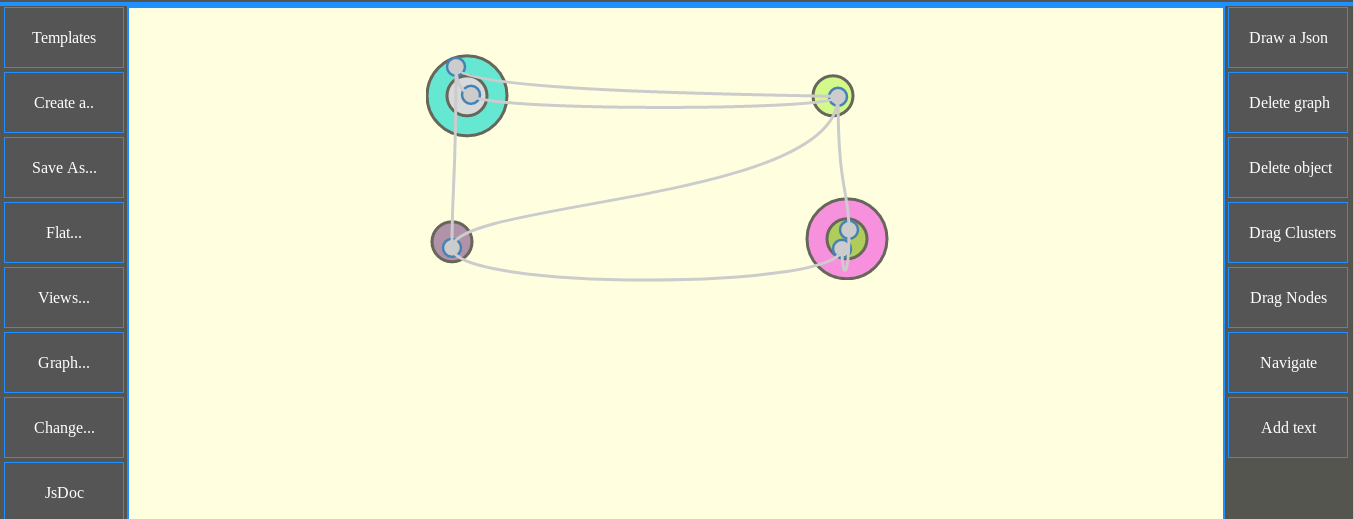
\includegraphics[width=0.8 \linewidth]{figure/changeRad}
	\end{center}
	\caption{operazione di cambiamento del raggio dei cluster da parte dell'utente\label{fig:changeRad}}
\end{figure}
\newline
Come già accennato ai cluster è assegnato un colore. Questo è di notevole importanza essendo un principio fondamentale per la rappresentazione, espresso anche nel capitolo relativo alle primitive della visualizzazione. Ad ogni cluster $\mu$ viene attribuito un valore random una volta che esso è stato aggiunto all'oggetto \textit{ClusteredGraph} e deve esser rappresentato. L'utente può cambiare questa tipologia di colorazione in due modi di seguito illustrati.\\
Il primo è quello di cambiare palette di lavoro, avendo così a disposizione tre colorazioni diverse che si riferiscono a tutte le sfumature facenti parte di quella particolare tonalità. Quando l'utente sceglierà di lavorare su una precisa tonalità per il prossimo numero indefinito di cluster il sistema imposterà alcuni valori esadecimali fissi per poter avere una scala di colori che richiami solo la tonalità richiesta dall'utente. Riprendendo nuovamente il grafo mostrato nella figura \figurename~\ref{fig:graphView} si può notare come essendo completamente casuale possono capitare anche colori non appariscenti o comunque non molto gradevoli all'occhio umano per questo l'utente mediante questa funzione potrà, a puro titolo di esempio, trasformarlo nel grafo mostrato nella \figurename~\ref{fig:changePalette}.
\begin{figure}[!htb]
	\begin{center}
		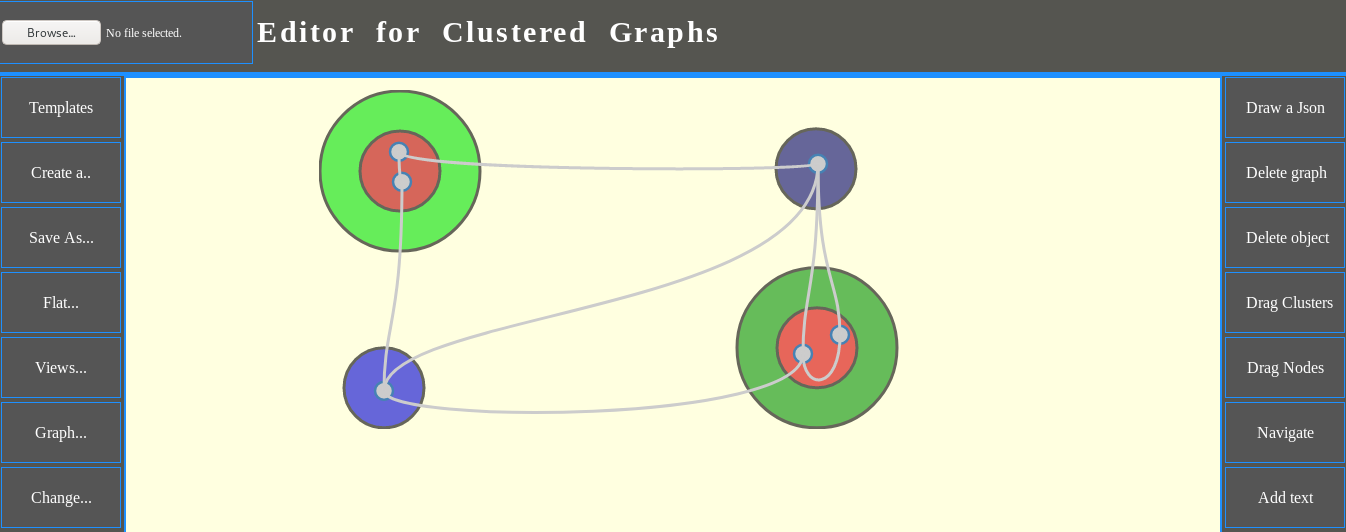
\includegraphics[width=0.8 \linewidth]{figure/changePalette}
	\end{center}
	\caption{impiego di Palette diverse da quella di default da parte dell'utente\label{fig:changePalette}}
\end{figure}
\newline
In questo modo è possibile anche catalogare e categorizzare in gruppi di cluster in base alla loro colorazione.
Con il secondo metodo realizzato, l'utente ha la possibilità di sostituire il colore assegnato ad un singolo cluster. In questo caso il sistema chiederà all'utente di inserire il valore esadecimale scelto per il colore. Una volta inserito verrà chiesto all'utente di decidere l'oggetto a cui applicare tale modifica.\\
L'editor è predisposto per lavorare su un numero moderatamente grande di cluster e di oggetti in generali. Per questo può esser utile aggiungere sul piano di lavoro etichette o comunque descrizioni degli oggetti che sono stati rappresentati. A titolo di esempio si può porre il caso in cui ogni cluster debba rappresentare un particolare oggetto o comunque si abbia bisogno un aiuto descrittivo su cosa rappresenti un particolare elemento oppure risulta necessario lasciare dei brevi commenti per essere visualizzati tra una sessione di lavoro e l'altra sullo stesso cluster. Questi problemi sono stati risposti dando la possibilità all'utente di poter richiedere al sistema un spazio in cui scrivere queste descrizioni per un particolare elemento del grafo clusterizzato. Una volta scritto il commento il sistema chiederà all'utente di selezionare l'oggetto a cui questa stringa sarà legata. Una volta visualizzata, la posizione all'interno della visualizzazione della stringa dipenderà dalle coordinate dell'oggetto associato di modo che in caso di modifica, spostamento o cancellazione, la posizione del testo verrà modificata e/o eliminata.\\
Un esempio di utilizzo, facendo ancora una volta riferimento alla \figurename~\ref{fig:graphView} del capitolo precedente, potrebbe essere quello riportato nella \figurename~\ref{fig:addText}.\\
\begin{figure}[!htb]
	\begin{center}
		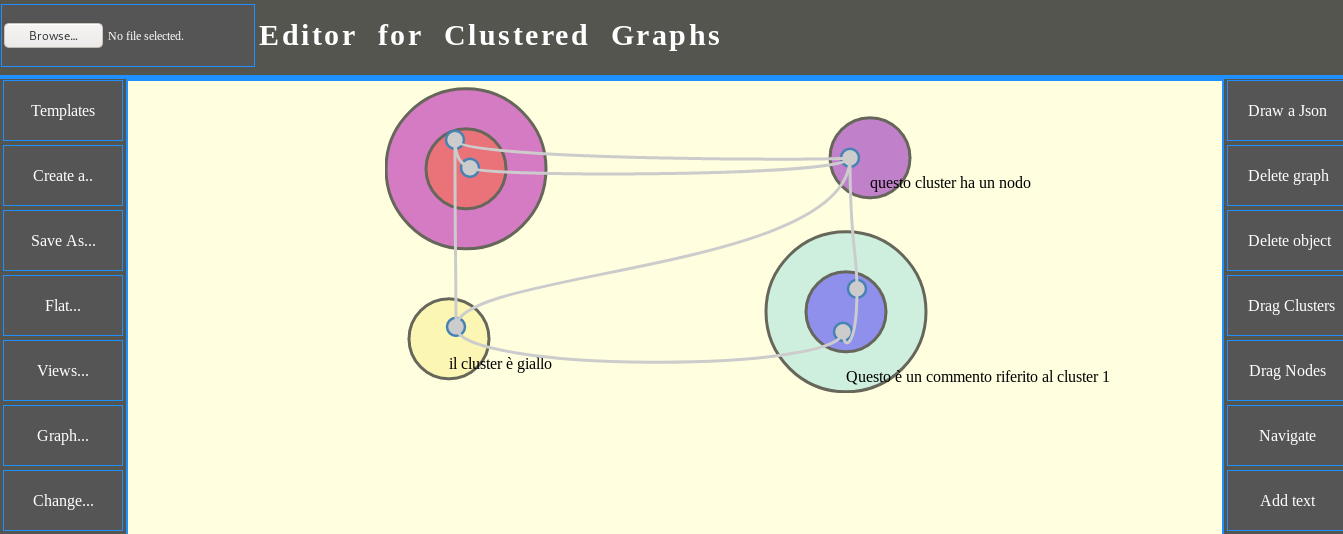
\includegraphics[width=1 \linewidth]{figure/addText}
	\end{center}
	\caption{aggiunta di commenti da parte dell'utente\label{fig:addText}}
\end{figure}
\newline
Nella figura i commenti visualizzati sono a puro titolo di esempio, ma basti pensare alla possibile utilità nel caso in cui si debba lavorare con decine di oggetti magari divisi in sottosezioni differenziate per colore ed in cui ogni raggruppamento ha uno specifico obiettivo che deve essere trasmesso da un utente ad un altro.
\section{navigazione}
La navigazione di una rappresentazione risulta essere una delle principali primitive per la visualizzazione come visto anche nel capitolo riferito proprio alle stesse.\\
Una buona visualizzazione deve poter dare all'utente la possibilità di navigare all'interno del piano di lavoro.\\
Non è però possibile modificare e navigare contemporaneamente in quanto risulterebbe difficoltoso e poco efficiente poter modificare un oggetto quando si sta eseguendo ad una operazione di focus su una particolare sezione di un grafo. Per questo, nel momento in cui l'utente ha necessità di eseguire queste operazioni relative ad uno zoom che sia semantico o non, dovrà prima richiedere al sistema di entrare in una modalità che può essere definita "\textit{navigate-view}". Entrando per la prima volta durante una stessa sessione all'interno di questa modalità sarà visualizzato un messaggio di aiuto per l'utente, come mostrato nella figura \figurename~\ref{fig:navMessage}, che indicherà le operazioni eseguibili in questa modalità.\\
\begin{figure}[!htb]
	\begin{center}
		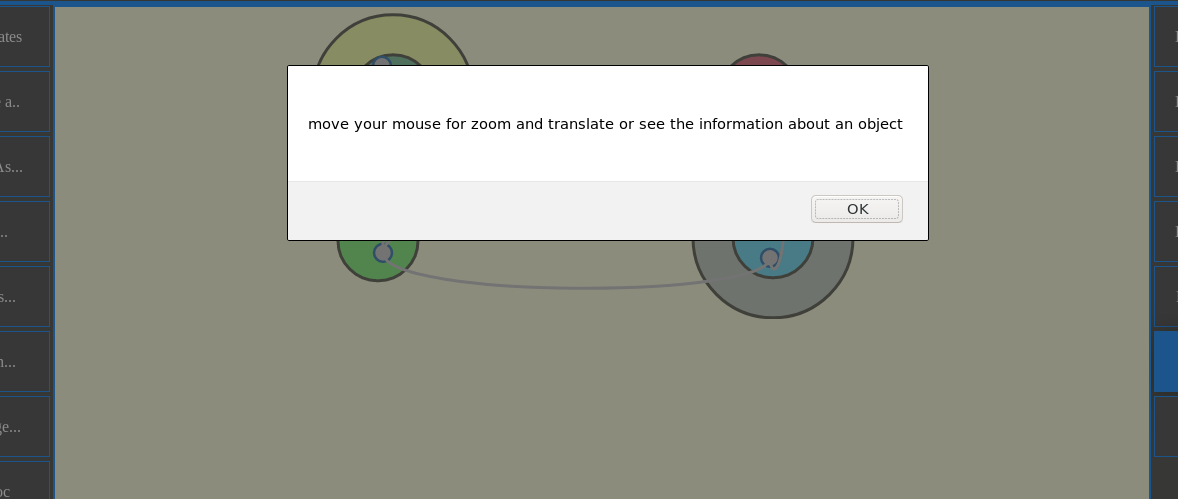
\includegraphics[width=1 \linewidth]{figure/navMessage}
	\end{center}
	\caption{Messaggio di aiuto al primo accesso dell'utente alla navigate-view\label{fig:navMessage}}
\end{figure}
\newline
Spostandosi sul piano di lavoro sarà possibile eseguire le primitive di traslazione e di zoom-in/out dell'intera rappresentazione del grafo clusterizzato come mostrato nella \figurename~\ref{fig:zoomGraph} in cui si sono eseguite le operazioni di traslazione e zoom-In rispetto alla rappresentazione della \figurename~\ref{fig:graphView}.
\begin{figure}[!htb]
	\begin{center}
		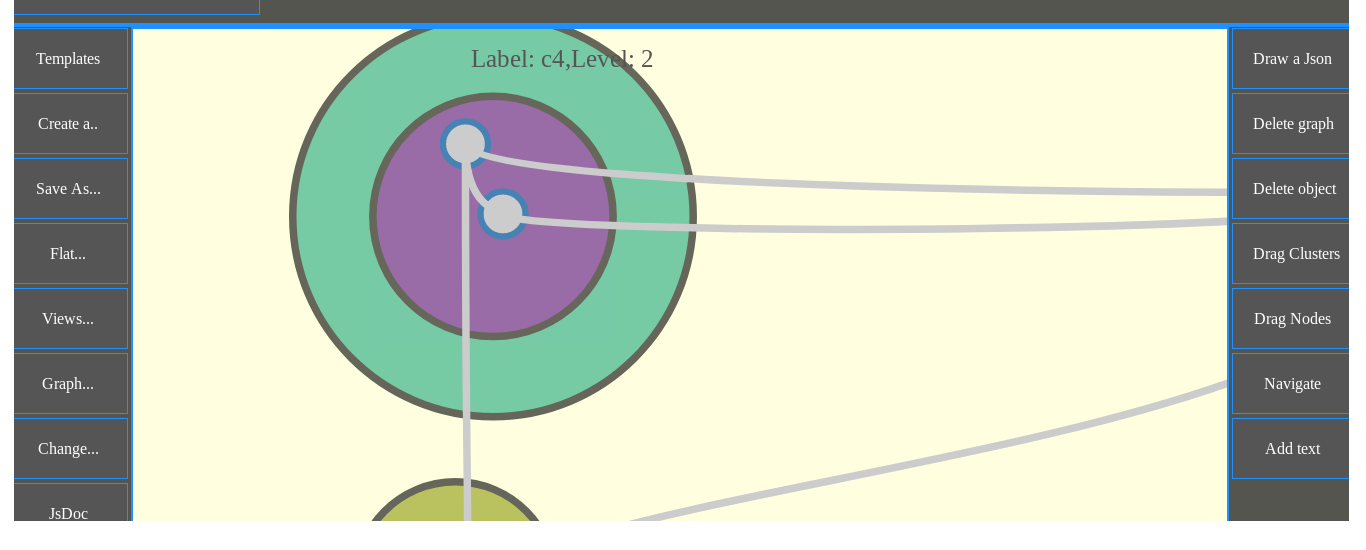
\includegraphics[width=1 \linewidth]{figure/zoomGraph}
	\end{center}
	\caption{zooming di un grafo nella navigate-view\label{fig:zoomGraph}}
\end{figure}
\newline
In questa modalità di visualizzazione inoltre passando sopra un oggetto sarà mostrato uno zoom semantico a schermo per dare più attenzione all'elemento. In particolare questo focus dipenderà dal tipo di oggetto evidenziato come mostrato di seguito:
\begin{itemize}
	\item \textbf{Nodo}: il raggio $r_n$ verrà moltiplicato per una costante e verrà visualizzata, in alto a destra, la sua etichetta e l'id del suo cluster di appartenenza;
	\item \textbf{Cluster}: il raggio $r_c$ verrà moltiplicato per una costante e verrà visualizzata la sua etichetta insieme al livello e alla lista di nodi che possiede al suo interno;
	\item \textbf{Arco}: saranno visualizzati gli id dei nodi che l'arco collega ovvero i suoi attributi \textit{source} e \textit{target}.
\end{itemize}
Gli attributi evidenziati saranno poi eliminati una volta che l'utente sposterà il cursore verso un oggetto diverso o verso il piano di lavoro, così da poter lasciare la possibilità al sistema di poter evidenziare un altro oggetto o di proseguire con la sessione di lavoro una volta uscito dalla \textit{navigate-view}.\\

\section{Semplificazione}
%%citare titto
Definite e chiarite le riduzioni polinomiali nel capitolo 6 si passa ora alla realizzazione. Per semplicità si è scelto di utilizzare una sola delle due tipologie di semplificazioni. In particolare questa scelta è ricaduta sulla riduzione da grafo clusterizzato $C$ in grafo Flat $C_f$.
L'utente, mediante una interazione su un bottone On/Off, potrà in qualunque momento richiedere al sistema di eseguire la semplificazione analizzata. Si è scelto di dare la possibilità all'utente di poter tornare alla visualizzazione precedente la trasformazione dei dati di modo da poter continuare la sessione e vedere potenziali differenze tra grafi clusterizzati e le loro riduzioni.\\
Lavorando nella visualizzazione a grafo, ovvero la \textit{graph-view}, ed avendo ultimato una prima analisi l'utente chiederà al sistema di eseguire la riduzione. Il sistema risponderà eseguendo l'algoritmo mostrato schematicamente nella \figurename~\ref{fig:flatAlg} e riportato di seguito in maniera semplificata. Alla base, l'algoritmo di riduzione in grafo clusterizzato flat è composto dai seguenti step:
\begin{itemize}
	\item \textbf{Step 0} Inizializzazione;
	\item \textbf{Step 1} Creazione cluster sostitutivi;
	\item \textbf{Step 2} Creazione dei nodi aggiuntivi;
	\item \textbf{Step 3} Sostituzione archi con percorsi;
	\item \textbf{Step 4} visualizzazione della classe \textit{clusteredGraph} ora resa Flat.
\end{itemize}
\begin{figure}[!htb]
	\begin{center}
		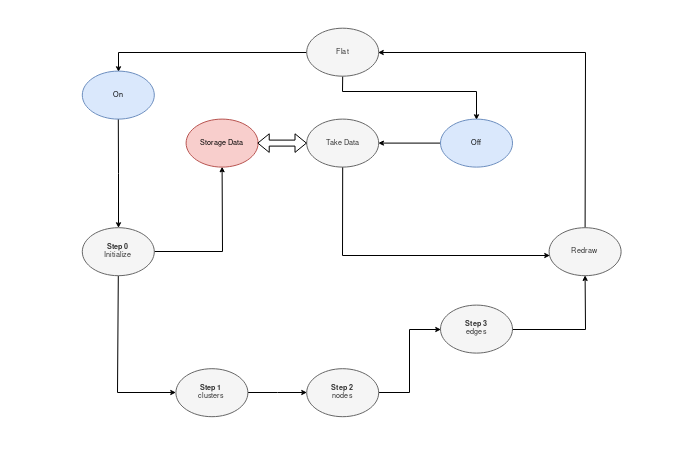
\includegraphics[width=1 \linewidth]{figure/flatAlg}
	\end{center}
	\caption{Struttura semplificata dell'algoritmo di flattizzazione \label{fig:flatAlg}}
\end{figure}
Nella fase di inizializzazione il sistema prima di eseguire qualunque cambiamento sugli oggetti creati e/o importati dall'utente provvederà ad eseguire una copia di questi dati per poter ritornare, se richiesto da una interazione utente, ai valori pre-riduzione e continuarne la modifica. Successivamente vengono create delle liste contenenti solo ed esclusivamente nodi e cluster del grafo su cui eseguire la riduzione. Gli elementi contenuti nella lista dei nodi saranno quelli con archi uscenti dal cluster e gli elementi della lista dei cluster saranno quelli con livello $l>2$.\\
Superata la fase di inizializzazione si passa alla trasformazione dei dati. Nello step 1 $\forall$cluster $\mu_i, \forall i=0,...,clusters.length$, con $clusters$ uguale alla lista dei cluster da cambiare inizializzata nello step 0, $\mu_i$ verrà eliminato ed al suo posto saranno inseriti due oggetti cluster $X$ o $Y$ che possiederanno come attributo label le rispettive etichette $\mu_i\_X$ e $\mu_i\_Y$.\\ 
Creati i cluster si passa poi allo step 2, ovvero alla creazione dei nodi aggiuntivi. In particolare $\forall$nodo $n_i, \forall i=0,...,nodes.length$ con nodes uguale alla lista dei nodi da cambiare inizializzata nello step 0, si creeranno due nodi $n_{i,j}\_X$ ed $n_{i,j}\_Y$ rispettivamente interni ai cluster creati prima, $\forall$ arco $e_j$, $\forall j=0,..., n_i.rotationScheme.length$ uscente dal cluster di appartenenza di $n_i$.\\
Nello step 3, creati cluster e nodi, si può passare alla rimozione degli archi inter-cluster e alla creazione del percorso $(source, e_\chi)(e_\chi, e\varphi) (e_\varphi, target)$
Terminate le trasformazioni il sistema concluderà con una operazione di visualizzazione della struttura dati mediante la rappresentazione riportata nella Tree-view come mostrato nella \figurename~\ref{fig:esempioTreeRidotto}.
\begin{figure}[!htb]
	\begin{center}
		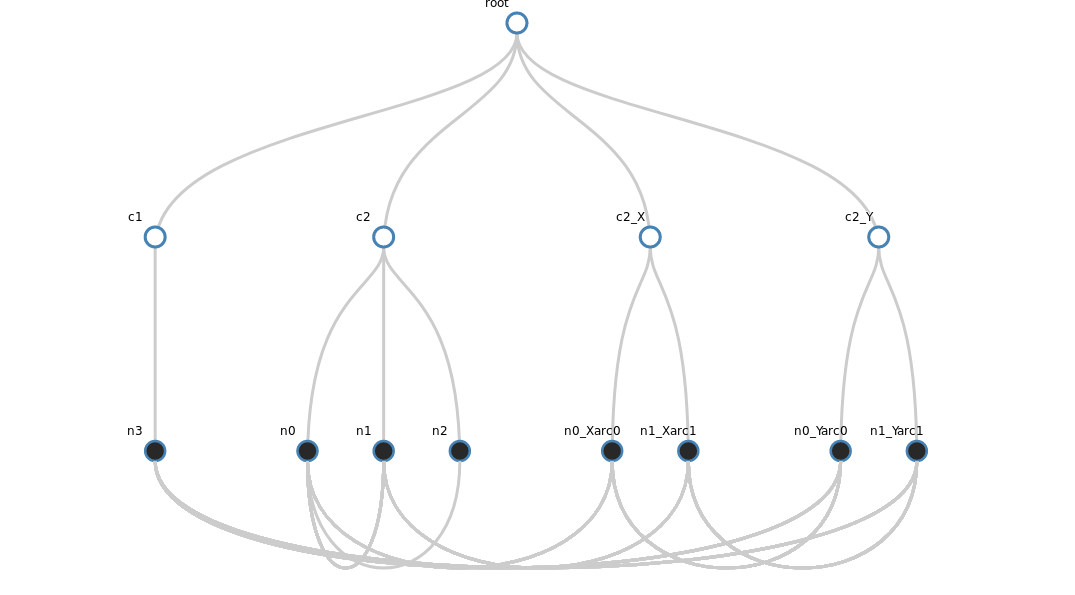
\includegraphics[width=1 \linewidth]{figure/esempioTreeRidotto}
	\end{center}
	\caption{Esempio della riduzione di un grafo clusterizzato nella Tree-View \label{fig:esempioTreeRidotto}}
\end{figure}
\newline
In qualunque momento l'utente potrà tornare alla visualizzazione del grafo non ancora ridotto e continuare il lavoro svolto.
Esempi reali di utilizzo di questa riduzione saranno visti nel dettaglio nel capitolo successivo in cui verranno utilizzate anche la maggior parte delle interazioni ed operazioni dell'utente. Sarà eseguita una simulazione reale di utilizzo e di test non solo inerente le connessioni tra gli oggetti che compongono il grafo clusterizzato ma anche sulla loro visualizzazione. Il sistema infine non pone alcun messaggio di errore nel caso in cui l'utente decida di effettuare una operazione di riduzione del grafo clusterizzato contenente errori nella sua definizione o nella sua visualizzazione in quanto non previsto che vengano eseguiti controlli su grafi erroneamente disegnati. Questo porta sicuramente a errori iniziali da parte dell'utente nell'approccio con il sistema ma dona anche la possibilità di eseguire qualunque operazione e grafo si decida di realizzare lasciando pieno controllo umano.

}